\section{Temporal Difference (TD)- Methods}\label{section:td-methods}
We now shift to the setting where we lack a model of the environment from which to derive 
an optimal policy. Instead, we are provided with sample trajectories, denoted as 
$\tau = (s_0, a_0, r_0, s_1, a_1, r_1, \dots)$, and must learn from these directly.

\subsection{Monte Carlo policy evaluation}\label{Monte Carlo policy evaluation}
Recall that the value function under a policy $\pi$ is defined as 
$V^{\pi}(s) = \mathbb{E}_{\pi}\left[G_t \mid s_t = s\right]$, where $G_t$ represents 
the discounted return starting from state $s$ at time $t$. The idea of Monte Carlo policy evaluation
is to approximate this expectation using Monte Carlo simulation. The core idea of Monte 
Carlo methods is to estimate an expectation, $\mathbb{E}_{p(x)}\left[f(x)\right] = \int p(x) f(x) \; dx$, 
by sampling from the distribution and averaging the results:
$$\mathbb{E}_{p(x)}\left[f(x)\right] = \int p(s)f(x) dx \approx \frac{1}{N} 
\sum_{x_i \sim p(x)} f(x_i)$$
This translates to sampling random episodes or trajectories under the policy $\pi$ 
and averaging the returns observed for each state to approximate $V^{\pi}(s)$. 
There are two primary approaches to compute this estimate: First-Visit Monte Carlo and Every-Visit Monte Carlo.
These methods differ in how they handle state visits within an episode and update the value estimates. 
The First-Visit approach updates the estimate only the first time a state $s$ is encountered at a timestep $t$ 
in an episode. In contrast, the Every-Visit approach updates the estimate for every occurrence of a 
state across all timesteps in the episode. At their core, they work as follows:

\begin{algorithm}[H]
  \large
    \caption{Monte Carlo Policy Evaluation }\label{MCPE}
    \begin{algorithmic}
        \STATE $N(s)\gets 0, G(s)\gets 0 \; \forall s \in S$
        \FOR{}
        \STATE sample episode $i = s_{i,1},a_{i,1},r_{i,1},s_{i,2},a_{i,2},r_{i,2},\dots,s_{i,T_i},a_{i,T_i},r_{i,T_i}$ \vskip 5pt
        \STATE define $G_{i,t} = r_{i,t}+ \gamma  r_{i,t+1} + \gamma^2  r_{i,t+2} + \dots +  \gamma^{T_i -1}  r_{i,T_i} $ as the return from time step $t$ onwords in the $i$th episode \vskip 5pt
        \FOR{$t \in T_i$} \vskip 3pt

        \STATE \tikzmk{A} \textcolor{red}{First-Visit Monte Carlo} 
        \STATE \textbf{if} this is the first time t that state s is visited in episode i
        \STATE
        \tikzmk{B}\boxit{mypink} 
        \STATE \tikzmk{A} \textcolor{blue}{Every-Visit Monte Carlo}
        \STATE state $s$ is being visited at time step $t$ in episode $i$
        \STATE
        \tikzmk{B}\boxit{myblue}
        \STATE increment counter of total visits $N(s) = N(s)+1$
        \STATE  $V^{\pi}(s)= V^{\pi}(s) + \alpha(G_{i,t}- V^{\pi}(s))$ \COMMENT{for $\alpha = \frac{1}{N(s)}$ equal to running average see \eqref{eq:running_avg}}
        
        %\STATE \tikzmk{A} \textcolor{red}{First-Visit Monte Carlo} 
        %\IF{this is the first time t that state s is visited in episode i}
        %\STATE increment counter of total first visits : $N(s)= N(s)+1$
        %\STATE increment total return $G(s) = G(s)+ G_{i,t}$
        %\STATE update estimate $V^{\pi}(s)= G(s)/N(s)$
        %\ENDIF
        %\STATE
        %\tikzmk{B}\boxit{mypink} 
        
        %\STATE \tikzmk{A} \textcolor{blue}{Every-Visit Monte Carlo}
        %\STATE state $s$ is being visited at time step $t$ in episode $i$
        %\STATE increment counter of total visits $N(s) = N(s)+1$
        %\STATE increment total return $G(s) = G(s)+ G_{i,t}$
        %\STATE update estimate $V^{\pi}(s)= G(s)/N(s)$
        %\STATE
        %\tikzmk{B}\boxit{myblue}
        
        %\STATE \tikzmk{A} \textcolor{black!70!green}{Incremental Monte Carlo}
        %\STATE state $s$ is being visited at time step $t$ in episode $i$
        %\STATE increment counter of total visits $N(s) = N(s)+1$
        %\STATE  $V^{\pi}(s)= V^{\pi}(s) + \alpha(G_{i,t}- V^{\pi}(s))$
        %\STATE
        %\tikzmk{B}\boxit{mygreen}
        \ENDFOR
        \ENDFOR

    \end{algorithmic}
\end{algorithm}
Convergence can be guaranteed depending on the choice of $\alpha$, provided the 
following conditions are satisfied:
\begin{itemize}
\item $\sum_{n=1}^{\infty} \alpha_n(s,a) = \infty \;\forall (s,a)$
\item $\sum_{n=1}^{\infty} \alpha_n^2(s,a) < \infty \;\forall (s,a)$            
\end{itemize}
The sample average method, using $\alpha_n = \frac{1}{n}$, fulfills these requirements. 
Additionally, it’s worth noting that the First-Visit Monte Carlo method is an unbiased 
estimator, whereas the Every-Visit Monte Carlo method is both unbiased and consistent
(meaning $\forall \epsilon > 0: \lim\limits_{n\rightarrow\infty} P(|V_n^{\pi}-V|> \epsilon)= 0$).\newline
The problem with the Monte Carlo estimator is that it is a high variance estimator, because if the 
policy or the environment is highly stochastic, the total return $G_t$ from a state can vary a lot 
even if you start from the same state. So, you're 
averaging a bunch of noisy, random returns = variance.
Reducing the variance can require a lot of data. Therefore, in cases where data is 
expensive to obtain MC may be impractical. Another 
disadvantage is that it only works if we have an episodic setting, which makes it 
very sample inefficient because we have to wait for the whole episode to end before we can 
compute the returns. But a nice feature is that it does not require the model to be 
Markov.

\subsection{Temporal Difference Learning}
Temporal Difference (TD) Learning combines the Monte Carlo method with dynamic programming 
which is used in the Value- and Policy-Iteration algorithms. This model-free technique is applicable
to both episodic and non-episodic environments. It updates the value function $V$ immediately after
each transition tuple $(s, a, r, s')$, with an update rule resembling that of incremental 
Monte Carlo methods:
$$V^{\pi}(s)= V^{\pi}(s) + \alpha(\underbrace{[r+ \gamma V^{\pi}(s')]}_{\text{TD target}}- V^{\pi}(s))$$
This version is known as TD(0), as it uses a one-step lookahead/ one-step return—for updating the value estimates.
\vspace{-0.2cm}
\begin{algorithm}[H]
 % \large
    \caption{Temporal Difference (TD(0)) Learning Algorithm }\label{TD_learning_algo}
    \begin{algorithmic}
        \STATE $V_0^{\pi}(s)\gets 0, \forall s \in S$
        \STATE Loop for each episode:
        \STATE \quad init. s
        \STATE \quad Loop 
        \STATE \qquad sample tuple $(s,a,r,s')$ from $\pi$
        \STATE \qquad $V^{\pi}(s)= V^{\pi}(s) + \alpha(r+ \gamma V^{\pi}(s'))- 
        V^{\pi}(s))$
        \STATE \qquad $s \gets s'$
        \STATE \quad until s is terminal
    \end{algorithmic}
\end{algorithm}
A key limitation of this approach is its inability to directly support policy improvement 
(see algo. \ref{policy improvement}). To compute the Q-values, we rely on the dynamics model, 
but such a model is unavailable in a model-free setting:
$$Q^{\pi_i}(s,a) \ \gets R(s,a) \ + \gamma \sum_{s'}{\color{red}p(s'|s,a)} V^{\pi_i}(s')$$
To address this, we shift to learning the Q-function directly instead of the value function, 
enabling policy improvement without dependence on the dynamics model.
%Recall that the goal is to choose actions that maximise expected future reward. But 
%n order to do this, we need to try out actions in order to know if they are 
%beneficial or not. This trade off of exploration vs exploitation has been already 
%addressed in k-armed-bandit chapter. With the following algorithms we will see how 
%this idea also plays a role.  

\subsection{Generalized Policy Improvement}
The first algorithm we’ll look at is Monte Carlo Online Control, which builds on 
Monte Carlo Policy Evaluation by incorporating updates to the Q-values.
\begin{algorithm}[H]
  %\large
    \caption{Monte Carlo Online Control}\label{Monte Carlo online control}
    \begin{algorithmic}
        \STATE $N(s,a)\gets 0, Q(s,a)\gets 0 \; \forall (s,a) \in S \times A$
        %\STATE $\epsilon \gets 1, k \gets 1$
        \FOR{(over episodes)}
        \STATE sample episode $i = s_{i,1},a_{i,1},r_{i,1},s_{i,2},a_{i,2},r_{i,2},\dots,s_{i,T_i},a_{i,T_i},r_{i,T_i}$ according to $\pi$ 
        \STATE define $G_{i,t} = r_{i,t}+ \gamma  r_{i,t+1} + \gamma^2  r_{i,t+2} + \dots +  \gamma^{T_i -1}  r_{i,T_i} $ 
        %as the return from time step $t$ onwords in the $i$th episode 
        \FOR{$t \in T_i$}
        \IF{First-Visit // Every-Visit}
        \STATE $N(s,a)= N(s,a)+1$
        \STATE $Q(s,a) = Q(s,a)+ \frac{1}{N(s,a)}(G_{i,t}-Q(s,a))$
        \STATE $\pi(s) \gets \argmax\limits_{a'} Q(s,a')$
        \ENDIF
        \ENDFOR
        %\STATE $k\gets k+1,$
        %\STATE $\epsilon \gets \frac{1}{k}$
        \ENDFOR
    \end{algorithmic}
\end{algorithm}
The Monte Carlo Online Control algorithm \footnote{ Monte Carlo Online Control isn’t sourced from the KIT lecture; it think i got it from Stanford’s CS234 course, so feel free to skip it.} converges to the optimal state-action 
value function $Q^*$ if the two conditions are fulfilled:
\begin{itemize}
\item Every state-action pair $(s, a)$ is visited infinitely often, expressed as
$\lim\limits_{i \to \infty} N_i(s, a) \to \infty$.
\item The behavior policy (the policy guiding actions in the environment) converges
to a greedy policy with probability 1, i.e., $\lim\limits_{i \to \infty} \pi(a|s) \to \arg\max_a Q(s, a)$.
\end{itemize}
These conditions are sometimes referred to as the ''Greedy in the Limit with Infinite Exploration``
(GLIE \label{glie}) property.

\subsubsection{TD-Learning with Q-Values}\label{sarsa and q learning}
Next, we will examine two variants of Temporal Difference (TD) Learning that update 
Q-values rather than value functions: SARSA and Q-Learning. While these methods are 
nearly identical, they only differ in their Q-value update rules.\newline
We begin with SARSA, the on-policy variant. In SARSA, the next action used to compute
the Q-value is determined by the current policy.
\begin{algorithm}[H]
  \large
    \caption{SARSA (on-policy TD control)}\label{Sarsa}
    \begin{algorithmic}
        \STATE $Q(s,a)\gets 0, \forall (s,a) \in S \times A$
        \STATE Loop for each episode:
        \STATE \quad init. s
        \STATE \quad choose a from s using policy derived from Q(e.g., $\epsilon-$greedy)
        \STATE \quad Loop for each step of episode
        \STATE \qquad take action $a$, observe $r,s'$ 
        \STATE \qquad choose $a'$ from $s'$ using policy derived from Q(e.g., $\epsilon-$greedy)
        \STATE \qquad $Q(s,a) \gets Q(s,a) + \alpha[r+\gamma Q(s',a')-Q(s,a)] $
        \STATE \qquad $s \gets s',a \gets a'$
        \STATE \quad until s is terminal
    \end{algorithmic}
\end{algorithm}
Q-Learning closely resembles SARSA, but operates off-policy due to the difference in 
its Q-value update rule:
$$Q(s,a) \gets Q(s,a) + \alpha[r+\gamma \;{\color{red}\max\limits_{a'}}\;Q(s',a')-Q(s,a)] $$
The $\max$ operator is what makes Q-Learning off-policy. Rather than sticking to the current 
policy to select the next action, it greedily chooses the action with the highest Q-value, 
diverging from the policy being followed. Both SARSA and Q-Learning can converge to the optimal solutions 
provided they satisfy the GLIE condition (see \ref{glie}) and the step sizes $\alpha_t$ meet the following two
criteria:
\begin{itemize}\label{robbins munro}
\item $\sum_{n=1}^{\infty} \alpha_n(s,a) = \infty \;\forall (s,a)$
\item $\sum_{n=1}^{\infty} (\alpha_n(s,a))^2 < \infty \;\forall (s,a)$
\end{itemize}
But there is still a problem with the algorithms shown here. They only work when
we can store all the values in tables. In fact, every algorithm so far only works if 
we can store the values in tables. For systems with many states and actions, this is 
a computational burden. And also the conditions for GLIE are somewhat impossible to 
fulfil if we have too many states and actions. Instead, we want a more compact 
representation that generalises across states or states and actions.

\subsection{Function Approximation for policy evaluation}
Rather than relying on tabular representations, we now use parametrized Q or V functions.
These can range from simple linear models to complex neural networks. The algorithms introduced
earlier remain mostly unchanged, except that we now also train a function approximator. 
Since the true Q-, V- or Reward-Function values are unavailable during training, we rely on approximated
targets as labels. The most well-known function approximation algorithm is
the Deep Q-Learning (DQN) algorithm, defined as follows:
 \begin{algorithm}[H]
  \large
    \caption{Vanilla Deep-Q-Learning (DQN)}\label{vanilla_dqn}
    \begin{algorithmic}
    \STATE \textbf{Input} $\alpha$
    \STATE $\text{init } \omega , t = 0$
    \STATE init. s
    \STATE \textbf{Loop} for each episode:
    \STATE \quad choose a from s using policy derived from $Q_\omega(s,a)$
    \STATE \quad observe $r,s'$ 
    \STATE \quad $y_i = \left\{
\begin{array}{ll}
r & \text{episode terminated at step i+1} \\
r + \gamma \max\limits_{a'}Q_\omega(s',a') & \, \textrm{otherwise} \\
\end{array}
\right. $
    \STATE \quad Do gradient descent step on $(y_i- Q_\omega(s,a))^2$ 
    \STATE \quad  $\omega \gets \omega + \alpha (y_i -  Q_\omega(s,a))\nabla_\omega  Q_{\omega}(s,a)$
    \STATE \quad $t \gets t+1$
    \STATE \quad $s \gets s'$
    \STATE \textbf{end loop}
    \end{algorithmic}
\end{algorithm}
One might argue that the gradient calculation of the loss contains an error, 
as $y_i$ also depends on $w$, yet its derivative seems to be missing. This is intentional.
The update rule incorporating the full gradient is known as the ''Residual Gradient Algorithm``. 
However, this approach minimizes the mean squared temporal difference error (MSTD), defined as:
$$ \text{MSTD} = \mathbb{E}_\pi\left[\left(r_t+\gamma \max\limits_{a'}Q_\omega(s',a')-Q_\omega(s, a)
\right)^2\right] \label{MSTD}$$ Minimizing the MSTD, however, does not guarantee Bellman optimality. 
Furthermore, the bias inherent in the residual gradient algorithm often results in 
suboptimal performance and slow convergence, making it less used in practice.\newline
An alternative approach to achieve Bellman optimality involves minimizing the Mean Squared 
Bellman Error (MSBE), defined as:
$$\text{MSBE} = \mathbb{E}_\pi\left[\left(r_t+ \gamma\mathbb{E}_{\color{red}p(\cdot|s, 
a)}[\max\limits_{a'}Q_\omega(s',a')]-Q_\omega(s,a)\right)^2\right] \label{MSBE}$$
However, computing the inner expectation in this formulation requires knowledge of the transition model,
which poses a significant challenge in the model free setting. One could simply use a single sample to 
estimate the expectation, which would effectively reduce the MSBE to the MSTD. However, there are also 
methods that employ two samples to address this, known as the double sampling approach. 
But these will not be discussed further.\newline Most of the time people will use the MSTD but don't take the gradient of 
the target values.

\subsubsection{Max Action Calculation}
To calculate the targets, we need to identify the action $a'$ with the highest Q-value for a given state. 
In discrete settings, the typical approach is to evaluate all possible actions and select the best one. 
However, this becomes highly inefficient and impractical for high-dimensional or continuous action spaces. 
There are several strategies to address this challenge, which we will explore in later chapters. Some of these include:

\begin{itemize}
    \item Gradient optimization on the Q-value network: One approach is to optimize the Q-value 
    network directly to find the best action. However, this introduces an additional inner loop 
    alongside the existing loop, which can significantly slow down the algorithm.
    
    \item Random shooting: This method involves sampling a set of actions $( a_1, \dots, a_n )$ 
    (e.g., uniformly), and selecting the best action from this set to maximize the Q-value when 
    calculating the target. While this approach is valid, it does not guarantee optimal results.
    
    \item Iterative stochastic optimization: This category includes methods such as the Cross-Entropy Method (CEM),
    Covariance Matrix Adaptation Evolution Strategy (CMA-ES), and others. These techniques operate similarly to random
    shooting but improve upon it by iteratively refining the action selection process to converge toward the optimal action. 
    (See Chapter~\ref{evo_strats} for more details.)

    \item Learning an approximate maximizer with a neural network: In this approach, a neural 
    network $ \mu_\beta $ is trained to approximate the action that maximizes the Q-value, i.e., 
    $ \mu_\beta \approx \argmax\limits_a Q_\psi(s,a) $.
\end{itemize}

\subsubsection{Improving DQN}
The vanilla DQN algorithm, as we have seen in algorithm \ref{vanilla_dqn}, is known to diverge 
very easily. There are two main problems. The first is that sequential states are 
highly correlated because some of the time steps are dependent on each other. The Q function would be 
updated many times for similar states while forgetting the Q values for other states 
(called catastrophic forgetting). In the DQN paper, they used a biologically 
inspired mechanism called experience replay (replay buffer). This approach stores past experiences and 
randomly samples mini-batches from the buffer during training, removing correlations in the observation sequence.\newline
The second challenge arises because the targets ($y_i$) are computed using the same model which is being trained. 
With each update, the target values shift alongside the Q-function, making the training process unstable. The solution is
to use a separate set of older weights to calculate the target values.
%A common choice for updating the target parameters is something similar to polynomial averaging.
%$$\omega' = \tau \omega'+(1-\tau)\omega$$

 \begin{algorithm}[H]
  \large
    \caption{Deep-Q-Learning (DQN) with Replay-Buffer and Target Networks \cite{mnih2013playingatarideepreinforcement}}\label{dqn}
    \begin{algorithmic}
    \STATE \textbf{Input} C,$\alpha,\tau$
    \STATE ${\color{cyan}D \gets \{\}}, \text{init } \omega, {\color{cyan}\omega'=\omega}, t = 0$
    \STATE init. s
    \STATE \textbf{Loop} for each episode:
    \STATE \quad choose a from s using policy derived from $Q_\omega(s,a)$
    \STATE \quad observe $r,s'$ 
    \STATE \quad {\color{cyan} store transition $(s,a,r,s')$ in replay buffer $D$}
    \STATE \quad {\color{cyan}sample random minibatch of tuples $(s_t,a_t,r_t,s_{t+1})$ from D}
    \STATE \quad \textbf{for} $i$ in minibatch \textbf{do} 
    \STATE \qquad $y_i = \left\{
\begin{array}{ll}
r_i & s_{i+1} \text{ is terminal} \\
r_i + \gamma \max\limits_{a'}Q_{\color{cyan}\omega'}(s_{i+1},a') & \, \textrm{otherwise} \\
\end{array}
\right. $
    \STATE \qquad Do gradient descent step on $(y_i- Q_\omega(s_i,a_i))^2$ for parameters
    \STATE \qquad  $w: \Delta w = \alpha (y_i -  Q_\omega(s_i,a_i))\nabla_\omega  Q_\omega(s_i,a_i) $
    \STATE \quad \textbf{endfor}
    \STATE \quad \textbf{if }$mod(t,C) == 0$ \textbf{then}
    \STATE \qquad {$\color{cyan}\omega' \gets \tau \omega'+(1-\tau)\omega $}
    \STATE \quad \textbf{endif}
    \STATE \textbf{end loop}
    \end{algorithmic}
\end{algorithm}

\subsubsection{Double Deep Q Learning}
The modified DQN algorithm works very well, but there is still a problem with this approach.
The issue is that the Q-values are overestimated, as depicted in Figure \ref{fig:ddqn}.
The problem lies in the max/argmax operator used for calculating the target values.
$$y_i= r_i + \gamma\;{\color{red}\max\limits_{a'}}\;Q_{\omega'}(s_{i+1},a') 
=  r_i + \gamma \;Q_{\omega'}(s_{i+1},{\color{red}\argmax\limits_{a'}}\;Q_{\omega'}(s_{i+1},a'))$$
The max operator is biased under noise, leading to overestimation. For random variables, this implies:
$$\mathbb{E}[\max{(X_1,X_2,\dots)}] \geq \max{(\mathbb{E}[X_1],\mathbb{E}[X_2],\dots)}$$
To understand this intuitively, imagine trying to determine the heaviest person in a group where everyone 
has the same true weight (e.g., 70kg), but the scale introduces random noise of $\pm$1kg. If you take the maximum
of these noisy measurements, it will almost always be greater than 70kg. Thus, the expectation of the maximum exceeds 
the maximum of the expectations, resulting in an upward bias.\newline 
Since the Q-values we use are estimates and inherently noisy, this max-based target leads to systematic overestimation during 
training. The solution is to use two different networks for action selection and value computation, i.e. the current network 
$\omega$ and the target network $\omega'$.
$$y_i = r + \gamma Q_{\beta}(s',\argmax\limits_{a'}\; Q_{\alpha}(s',a'))$$. 
\begin{figure}[H]
    \centering
    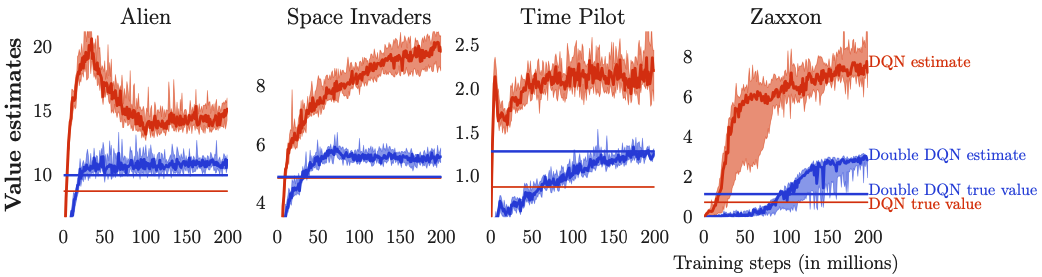
\includegraphics[width=\linewidth]{images/DDQN.png}
    \caption{Value estimates by DQN (orange) and Double DQN (blue) on some Atari games, from \cite{vanhasselt2015deepreinforcementlearningdouble}}
    \label{fig:ddqn}
\end{figure}

\subsubsection{Multi-Step Returns} \label{multi_steps}
In the versions of Q-Learning /DQN we've been looking at, a 1-step look-ahead is employed to compute the targets 
$$y = r + \gamma \max\limits_{a'}Q_\omega(s',a')$$
This results in low variance but a high bias, suggesting that the Q is likely 
wrong. \newline 
To address this, we can use n-step returns, which extend the target by rolling out the actual rewards over $n$
steps before bootstrapping from the Q-function:
$$y_t = r(s_t,a_t)+ \gamma r(s_{t+1},a_{t+1})+ \gamma^2  r(s_{t+2},a_{t+2})+\dots+\gamma^n\max\limits_{a'}Q_\omega(s_{t+n},a')$$
Conversely, an n-step look-ahead yields no bias but high variance. Therefore,
a trade-off has to be made. But n-step returns are not compatible with off-policy methods such 
as Q-learning, as it violates the definition of the Q-function, which is defined as 
the expected sum of future rewards if we start in state s and perform action a and 
then follow the policy. In the context of a two-step look-ahead, the target is defined as
$$y_t = r(s_t,a_t)+ \gamma r(s_{t+1},a_{t+1})+\gamma^2\max\limits_{a'}Q_\omega(s_{t+2},a')$$
Note that $s_t$ and $a_t$ may take on any value since their choice does not violate 
the definition. But it is necessary for $a_{t+1}$ to align with the policy in order 
to ensure that the condition is met. This, however, implies that the choice of 
$a_{t+1}$ is not entirely free, and consequently, the look a head is not off-policy. 
It is noteworthy that there exist multiple methods to circumvent this issue, which 
will not be delved into in this discussion.
%Finally, I would encourage you to look at the rainbow paper, which is a gateway to all sorts of dance techniques.

\subsection{Self-Test Questions}
 \begin{enumerate}
     
\sq{ What we mean by Monte Carlo estimates} $\rightarrow$ \ref{Monte Carlo policy evaluation}

\sq{ Why TD learning can be seen as a combination of MC and Dynamic 
Programming}\newline DP because we compute the value function iteratively starting 
from 0 for all states and MC because we sample an action in every iteration and use 
that action to compute the target $y_t$ for time step $t$. This target is then 
incorporated by moving average 

\sq{ What is the TD error ? }$V^{\pi}(s_t)= V^{\pi}(s_t) + \alpha 
\underbrace{([r_t+ \gamma V^{\pi}(s_{t+1})]- V^{\pi}(s_t))}_{\text{TD error}}$

\sq{ How Q-Learning works} $\rightarrow$ \ref{sarsa and q learning}

\sq{ What Value function approximation is}\newline We don't store the values in tables 
any more. Instead, we use parametrised function approximations of the V/Q-Function. 
Here we calculate the gradients of specific loss functions in order to update the parameters. 

\sq{ Why Q-Learning is not actual gradient ascent?} \newline There is no clearly defined 
objective since the targets are always changing since we also approximate them ourself.

\sq{ How to fix Q-learning for deep neural networks?}\newline
Use a replay buffer where we randomly select transitions to solve the problem that 
successive states are highly correlated. And use a separate target network to 
compute the targets to solve the problem that the targets would keep changing 
because they were computed by the same network that was supposed to learn the policy.

\sq{ Why do we get the over-estimation effect and how to fix it?}\newline
Under noise the max operator is biased to be larger than it should be. And since our 
estimate of Q is a noisy estimate this leads to the overestimation effect. We fix it by 
using the double DQN method. There we use two separate networks. The first one selects the 
(what it thinks) best possible action and the second one calculates the target by using the 
suggested action.

\end{enumerate}

\subsection{Resources}
Much of the content here on Deep Q-Learning is based on Sergey Levine’s CS 285: Lecture 8 \cite{CS285,CS285LevineYoutube}.